\documentclass[border=2mm]{standalone}
\usepackage{tikz}
\usepackage{helvet}
\renewcommand{\familydefault}{\sfdefault}
\usepackage{amsmath}

\usepackage{pgfplots}
\pgfplotsset{
tick label style = {font=\sansmath\sffamily}, compat=newest}

\begin{document}
\footnotesize

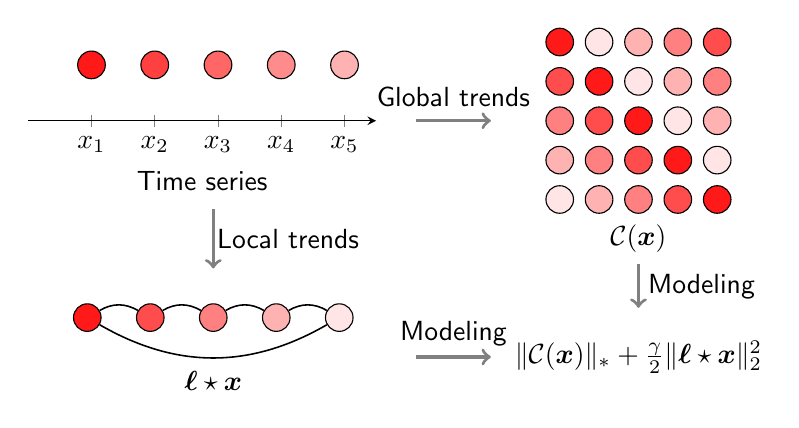
\begin{tikzpicture}
\begin{axis}[axis lines=left, enlargelimits=upper, domain=0:2, xmin=0, axis y line=none, xtick={1,2,3,4,5}, xticklabels={${x}_{1}$,${x}_{2}$,${x}_{3}$,${x}_{4}$,${x}_{5}$}, legend pos=outer north east, width=6cm, height=3.0cm, xlabel=Time series, xlabel near ticks, ylabel near ticks]

\addplot[only marks, mark size=5, color=red!90, draw=black] coordinates{(1,1)};
\addplot[only marks, mark size=5, color=red!75, draw=black] coordinates{(2,1)};
\addplot[only marks, mark size=5, color=red!60, draw=black] coordinates{(3,1)};
\addplot[only marks, mark size=5, color=red!45, draw=black] coordinates{(4,1)};
\addplot[only marks, mark size=5, color=red!30, draw=black] coordinates{(5,1)};

\end{axis}

\newcommand{\rightpos}{0.5}
\node at (5.4,0.8-\rightpos) {\color{black}Global trends};
\node (A) at (4.8,0.5-\rightpos) {};
\node (B) at (6,0.5-\rightpos) {};
\draw [->,very thick,gray] (A) edge (B);

\newcommand{\circpos}{0.25}

\node[circle,draw=black,fill=red!90,inner sep=0pt,minimum size=0.35cm] at (7-\circpos,1.5-\rightpos) {};
\node[circle,draw=black,fill=red!70,inner sep=0pt,minimum size=0.35cm] at (7-\circpos,1.0-\rightpos) {};
\node[circle,draw=black,fill=red!50,inner sep=0pt,minimum size=0.35cm] at (7-\circpos,0.5-\rightpos) {};
\node[circle,draw=black,fill=red!30,inner sep=0pt,minimum size=0.35cm] at (7-\circpos,0.0-\rightpos) {};
\node[circle,draw=black,fill=red!10,inner sep=0pt,minimum size=0.35cm] at (7-\circpos,-0.5-\rightpos) {};

\node[circle,draw=black,fill=red!10,inner sep=0pt,minimum size=0.35cm] at (7.5-\circpos,1.5-\rightpos) {};
\node[circle,draw=black,fill=red!90,inner sep=0pt,minimum size=0.35cm] at (7.5-\circpos,1.0-\rightpos) {};
\node[circle,draw=black,fill=red!70,inner sep=0pt,minimum size=0.35cm] at (7.5-\circpos,0.5-\rightpos) {};
\node[circle,draw=black,fill=red!50,inner sep=0pt,minimum size=0.35cm] at (7.5-\circpos,0.0-\rightpos) {};
\node[circle,draw=black,fill=red!30,inner sep=0pt,minimum size=0.35cm] at (7.5-\circpos,-0.5-\rightpos) {};

\node[circle,draw=black,fill=red!30,inner sep=0pt,minimum size=0.35cm] at (8-\circpos,1.5-\rightpos) {};
\node[circle,draw=black,fill=red!10,inner sep=0pt,minimum size=0.35cm] at (8-\circpos,1.0-\rightpos) {};
\node[circle,draw=black,fill=red!90,inner sep=0pt,minimum size=0.35cm] at (8-\circpos,0.5-\rightpos) {};
\node[circle,draw=black,fill=red!70,inner sep=0pt,minimum size=0.35cm] at (8-\circpos,0.0-\rightpos) {};
\node[circle,draw=black,fill=red!50,inner sep=0pt,minimum size=0.35cm] at (8-\circpos,-0.5-\rightpos) {};

\node[circle,draw=black,fill=red!50,inner sep=0pt,minimum size=0.35cm] at (8.5-\circpos,1.5-\rightpos) {};
\node[circle,draw=black,fill=red!30,inner sep=0pt,minimum size=0.35cm] at (8.5-\circpos,1.0-\rightpos) {};
\node[circle,draw=black,fill=red!10,inner sep=0pt,minimum size=0.35cm] at (8.5-\circpos,0.5-\rightpos) {};
\node[circle,draw=black,fill=red!90,inner sep=0pt,minimum size=0.35cm] at (8.5-\circpos,0.0-\rightpos) {};
\node[circle,draw=black,fill=red!70,inner sep=0pt,minimum size=0.35cm] at (8.5-\circpos,-0.5-\rightpos) {};

\node[circle,draw=black,fill=red!70,inner sep=0pt,minimum size=0.35cm] at (9-\circpos,1.5-\rightpos) {};
\node[circle,draw=black,fill=red!50,inner sep=0pt,minimum size=0.35cm] at (9-\circpos,1.0-\rightpos) {};
\node[circle,draw=black,fill=red!30,inner sep=0pt,minimum size=0.35cm] at (9-\circpos,0.5-\rightpos) {};
\node[circle,draw=black,fill=red!10,inner sep=0pt,minimum size=0.35cm] at (9-\circpos,0.0-\rightpos) {};
\node[circle,draw=black,fill=red!90,inner sep=0pt,minimum size=0.35cm] at (9-\circpos,-0.5-\rightpos) {};

\node at (8-\circpos,-1.0-\rightpos) {\color{black}$\mathcal{C}(\boldsymbol{x})$};

\node at (8.8-\circpos,-1.6-\rightpos) {\color{black}Modeling};
\node (E) at (8-\circpos,-1.2-\rightpos) {};
\node (F) at (8-\circpos,-2-\rightpos) {};
\draw [->,very thick,gray] (E) edge (F);

\node at (3.3,-1.5) {\color{black}Local trends};
\node (C) at (2.35,-1) {};
\node (D) at (2.35,-2) {};
\draw [->,very thick,gray] (C) edge (D);

\newcommand{\shift}{2.5}

\node[circle, draw = black, fill = red!90, minimum size = 0.35cm] (x1) at (0.75, 0-\shift) {};
\node[circle, draw = black, fill = red!70, minimum size = 0.35cm] (x2) at (1.55, 0-\shift) {};
\node[circle, draw = black, fill = red!50, minimum size = 0.35cm] (x3) at (2.35, 0-\shift) {};
\node[circle, draw = black, fill = red!30, minimum size = 0.35cm] (x4) at (3.15, 0-\shift) {};
\node[circle, draw = black, fill = red!10, minimum size = 0.35cm] (x5) at (3.95, 0-\shift) {};

\path [draw, line width = 0.2mm, -] (x1) edge [bend left] node [right] {} (x2);
\path [draw, line width = 0.2mm, -] (x2) edge [bend left] node [right] {} (x3);
\path [draw, line width = 0.2mm, -] (x3) edge [bend left] node [right] {} (x4);
\path [draw, line width = 0.2mm, -] (x4) edge [bend left] node [right] {} (x5);

\path [draw, line width = 0.2mm, -] (x1) edge [bend right] node [left] {} (x5);

\node at (2.35,-0.8-\shift) {\color{black}$\boldsymbol{\ell}\star\boldsymbol{x}$};

\node at (5.4,0.3-\shift-\rightpos) {\color{black}Modeling};
\node (G) at (4.8,0-\shift-\rightpos) {};
\node (H) at (6,0-\shift-\rightpos) {};
\draw [->,very thick,gray] (G) edge (H);

\node at (8-\circpos,-0-\shift-\rightpos) {\color{black}$\|\mathcal{C}(\boldsymbol{x})\|_{*}+\frac{\gamma}{2}\|\boldsymbol{\ell}\star\boldsymbol{x}\|_{2}^{2}$};

\end{tikzpicture}

\end{document}
